\chapter{Informed Multi-Task Learning}
\label{chap:mtl}
Based on our findings from the probing experiments, we now want to address the question on whether the knowledge obtained from probing can be leveraged to improve the BERT ranking model.

Thus, our new objective becomes re-ranking: Given a query $q$ and a set of candidate documents $C=\{c_i\}_{i=1}^{|C|} \subseteq D$, we want to learn a ranker $s: Q \times D \rightarrow \R$, such that for any two candidate documents $c, c' \in C$, it holds true that $s(q, c) > s(q, c')$ if $c$ is more relevant than $c'$, regarding $q$.\\
From our probing experiments we found that different properties are best captured around specific layers. Therefore, we want our experiment to satisfy the following criteria:
\begin{itemize}
    \item Exploit the fact that ranking properties emerge in intermediate layers.
    \item Use the knowledge on which layers capture what property best.
\end{itemize}
The main idea of our approach is to aid fine-tuning by infusing task knowledge into specific layers through \ti{multi-task learning}. We want to simultaneously learn ranking properties at the layers that we found to be best at capturing them, especially when being fine-tuned for ranking.

To achieve this, for each task, we first select a layer that we found to efficiently encode the corresponding  ranking property during probing. We then fine-tune the \ti{bert-base-uncased} model to perform ranking on the TREC2019 dataset. At the same time, we jointly learn classifiers on top of BERT's intermediate layer representations of the pre-selected layers, to predict the respective ranking properties.

\section{Model Architecture}
Given the intermediate layer representations of the pre-trained \ti{bert-base-uncased} model $\{H\lay i\}_{i=0}^{12}$, with $H\lay i = (h_1, h_2, \dots, h_{N})$ being the sequence of token embeddings at layer~$i$, for each task (\Cref{sec:tasks}), we select a layer based on the probing results. We then apply average pooling across the sequence dimension to retrieve a fixed size embedding:

\begin{equation}
    \tx{pool}(h_i, h_{i+1},\dots, h_j)= \frac{1}{j-i} \sum_{k=i}^j h_k
\end{equation}
In the case of tasks that require multiple spans, we first average along each span $(i,j) \in S$ and then concatenate the resulting vectors:

\begin{equation}
    \tx{multi-pool}(h_1, \dots, h_N) = \bigparallel_{(i, j) \in S}{\tx{pool}(h_i, h_{i+1},\dots, h_j)}
\end{equation}
Following the pooling we apply a simple MLP classifier of the form:

\begin{equation}
    \tx{MLP}(x) = \tx{ReLU}(x W^{(0)} + b^{(0)}) W^{(1)} + b^{(1)}
\end{equation}
Unlike the auxiliary tasks, ranking is performed by applying the same MLP to the first output embedding at the last layer of BERT which corresponds to the [CLS] token (See \citep{devlin-etal-2019-bert}).

\begin{figure}[!hb]
    \centering
    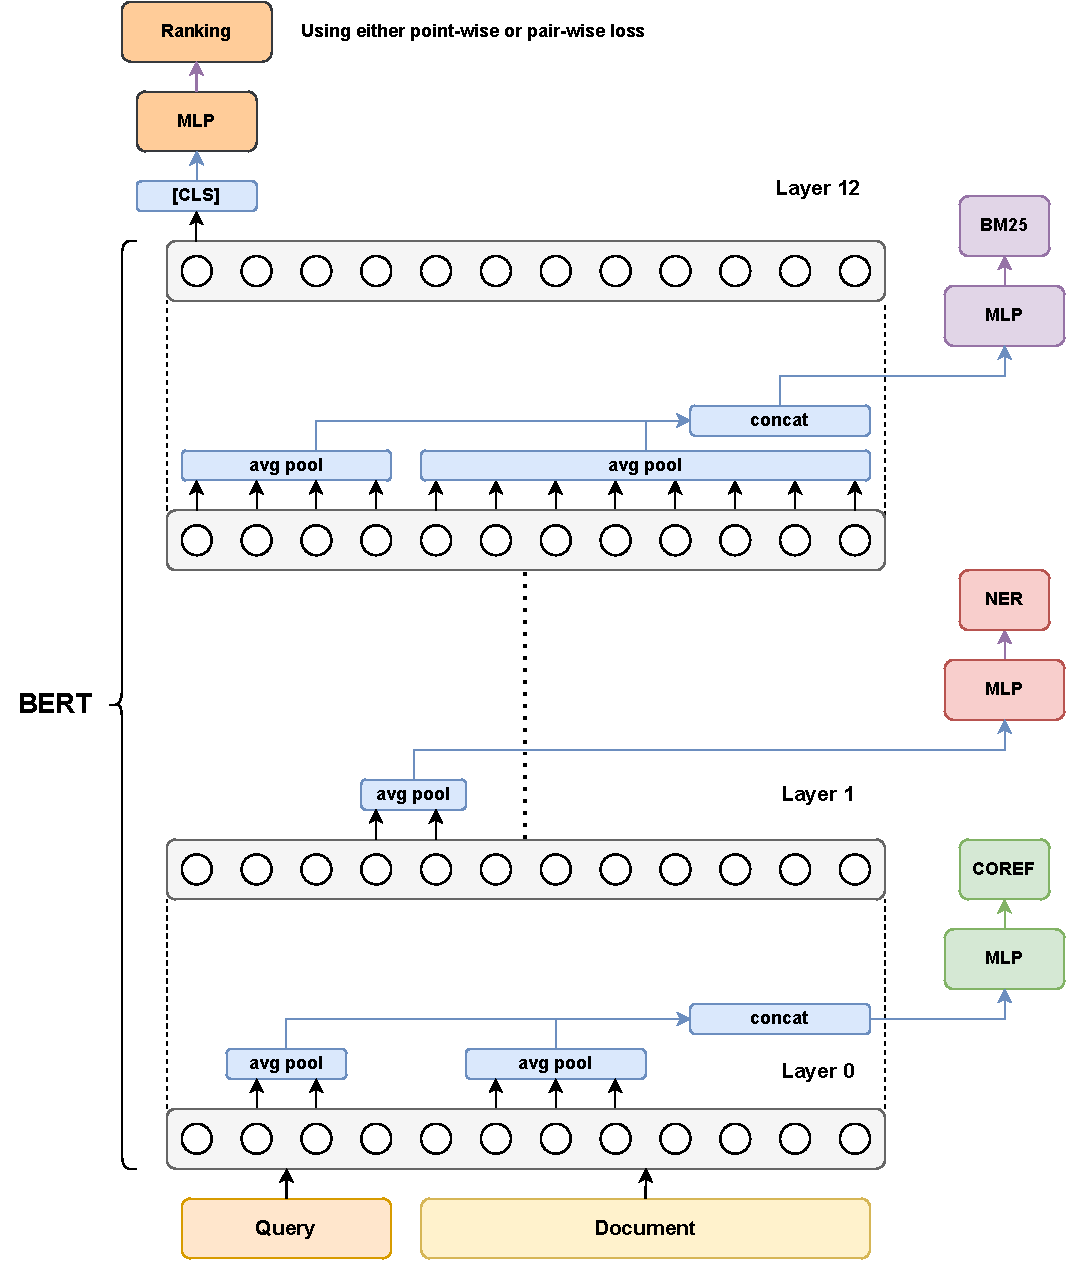
\includegraphics[width=.9\textwidth]{gfx/mtl/mtl-example}
    \caption{Exemplary instantiation of our MTL architecture with 3 additional tasks. The main objective \ti{ranking} is learned at the last layer, following the standard BERT fine-tuning approach. For each auxiliary task, a different MLP is applied at an intermediate layer. Note that, unlike during our probing, the parameters of BERT are no longer fixed and jointly optimized with all MLPs.}
    \label{fig:mtl}
\end{figure}

\section{Experimental Setup}
\subsection{Datasets and Sampling}
Because our objective is now re-ranking on TREC2019, we can no longer rely on the original probing datasets, as they were sampled from the test set and therefore would cause test set overlap. Instead, we sample new query-document pairs from the TREC2019 train set. Our sampling goes as follows: We uniformly sample $100$k train queries for each task. Then, for each query we retrieve $10$ documents from the corpus using BM25, resulting in a dataset size of $1$M samples which is approximately the size of the TREC2019 ranking dataset. Each task dataset is then constructed by applying the same procedure as in \Cref{sec:dataset_gen} and \Cref{sec:tasks}, to automatically generate labels.

We exclude the fact-checking task, as we do not have a straightforward way to automatically generate samples and the dataset itself is too small when compared to the other datasets. Furthermore, due to time constraints we do not include COREF when training more than $2$ tasks jointly.

\subsection{Training}
During training, we assemble mini-batches of size $32$, by sampling from the TREC2019 train set and all generated task datasets with a probability proportional to their size. As loss function we use the objective proposed in \citep{aghajanyan-etal-2021-muppet}:

\begin{equation}
    \label{eq:muppet}
    \mathcal{L}(y, \hat{y}) = \sum_{t \in \tx{tasks}} \frac{\textnormal{CE}(y_t, \hat{y}_t)}{\log c_t}
\end{equation}
where $c_t$ is the number of target classes and $y_t$, $\hat{y}_t$ are predictions and ground-truth labels with respect to task $t$, respectively. It scales each task loss, such that all losses would have equivalent values, if the class distribution were uniformly distributed, along with the predictions. Analogous to the probing experiments, regression tasks are cast to classification tasks by binning the targets into $k=10$ categories, so that $c_t$ is defined properly.
We train each model for up to a maximum of $100$ epochs and perform early stopping after $3$ epochs of no improvement in MAP on the TREC2019 validation set. As optimizer, we use Adam \citep{kingma2014adam} with a learning rate of 2e-6 and linearly increase the learning rate over the first $10k$ steps. Each task specific classifier has a hidden size of $128$ and dropout with rate $0.2$ is applied before each layer.

In addition to binary cross-entropy loss, we further experiment with a pair-wise margin loss for the ranking task:
\begin{equation}
    \tx{MarginLoss}(y^+, y^-) = \max(\lambda - y^+ + y^-, 0)
\end{equation}
where $\lambda=0.2$ is the margin and $y^+, y^-$ are the model's predictions for a relevant and non-relevant document, respectively.

Each model is trained on a server with $256$GB of system memory, using either a single Nvidia A100 or V100 GPU.


\section{Results}
\label{sec:mtl_results}
\subsection{Single Additional Task}
For runs in which a single additional task is introduced (\Cref{tab:single_runs}), we can observe a general improvement across the board. It also becomes apparent that the selection of layer which the additional task is trained on actually plays a role: For BM25, SEM and COREF, layer $12$ shows worse or equal performance for most metrics, when compared to layers that were selected based on our probing results. For instance, BM25 consistently outperforms the baseline at layers $5$ and $6$. However, at layer $12$ it performs significantly worse than the baseline. This coincides with our findings from probing where the final layer appears to be overspecialized and therefore less receptive for additional task information.

Interestingly, this does not apply to NER which, except from MRR, instead performs best at the final layer. We hypothesize that, due to the NER property having a rather flat distribution across layers (\Cref{fig:heatmap_comp_base}), infusing additional NER information might work equally well at most layers.

In terms of MAP, we also find NER to yield the highest benefit while the highest increase in MRR, NDCG and precision stems from the additional COREF task. Considering that probing showed the most absolute increase in COREF information when fine-tuning for ranking (\Cref{fig:abs_heatmap_comp_base}, \Cref{fig:abs_heatmap_comp_passage}), this might be additional evidence for coreference being a useful ability for a neural ranker to learn. Moreover, the performance of NER which seems to be closely related to COREF, suggests that entities in general play an important role for learning to rank.

\begin{table}[ht]
    \centering
    \begin{tabular}{lc|cccc|c}
        \hline
        \tf{Tasks}  & \tf{Layer} & \tf{MAP}   & \tf{MRR}   & \tf{NDCG@10} & \tf{P@10}  & \tf{avg}   \\ \hline\hline
        \tx{TREC}   & 12         & 0.436      & 0.926      & 0.678        & 0.784      & 0.706      \\ \hline
        \tx{+BM25}  & 5          & 0.437      & 0.947      & 0.682        & \tf{0.791} & 0.714      \\
        ~           & 6          & 0.439      & \tf{0.953} & \tf{0.690}   & 0.772      & 0.714      \\
        ~           & 12         & 0.420      & 0.912      & 0.659        & 0.749      & 0.685      \\ \hline

        \tx{+NER}   & 4          & \tf{0.447} & \tf{0.950} & 0.685        & 0.788      & \tf{0.717} \\
        ~           & 5          & \tf{0.444} & 0.934      & 0.680        & 0.772      & 0.708      \\
        ~           & 12         & \tf{0.447} & 0.944      & \tf{0.688}   & \tf{0.791} & \tf{0.717} \\ \hline
        \tx{+SEM}   & 1          & 0.436      & 0.934      & 0.682        & 0.784      & 0.709      \\
        ~           & 4          & 0.440      & 0.928      & 0.682        & 0.779      & 0.707      \\
        ~           & 12         & 0.436      & 0.928      & 0.669        & 0.774      & 0.702      \\ \hline
        \tx{+COREF} & 5          & 0.442      & \tf{0.965} & \tf{0.694}   & \tf{0.798} & \tf{0.725} \\
        ~           & 7          & 0.425      & 0.944      & 0.668        & 0.770      & 0.702      \\
        ~           & 12         & 0.442      & 0.948      & 0.681        & 0.788      & 0.715      \\
    \end{tabular}
    \caption{Test results for single additional task runs. The first row corresponds to a baseline that was solely trained on TREC2019. +[TASK] indicates multi-task training on TREC2019 and [TASK] simultaneously. The top 3 runs for each metric are highlighted in bold.}
    \label{tab:single_runs}
\end{table}

\subsection{Full Multi-task}
The results for the full multi-task runs are shown in \Cref{tab:multi_runs}. Surprisingly, all runs perform equal to or worse than the baseline, with a single exception being the layer combination $5,1,12$ on MRR. One hypothesis why this might be the case, is that the ranking task is simply overshadowed by the other tasks, since with this setup only $\frac{1}{4}$ of the dataset specifically addresses ranking. To test this hypothesis, we did perform another run where each additional task was limited to $200$k samples each. However, we could not observe any improvement from this approach.

Another hypothesis suggests that too many tasks start to conflict with one another, leading to hidden representations that are no longer coherent with each other and as a consequence, less useful for learning the ranking task. Interestingly, \citep{aghajanyan-etal-2021-muppet} found their multi-task learning setup to perform best when at least $10$ tasks were used, meaning it is also possible that $3$ additional tasks are simply not sufficient.

Nonetheless, we can still observe that selecting intermediate layers based on probing metrics generally results in higher performance than simply employing the additional task at layer $12$.

\begin{table}[ht]
    \centering
    \begin{tabular}{lc|cccc|c}
        \hline
        \tf{Tasks}        & \tf{Layers} & \tf{MAP}   & \tf{MRR}   & \tf{NDCG@10} & \tf{P@10}  & \tf{avg}   \\ \hline\hline
        TREC              & 12          & \tf{0.436} & 0.926      & \tf{0.678}   & \tf{0.784} & \tf{0.706} \\ \hline
        +BM25, +SEM, +NER & 5, 1, 12    & 0.425      & \tf{0.950} & 0.675        & 0.772      & 0.705      \\
        ~                 & 5, 4, 6     & 0.431      & 0.930      & 0.670        & 0.758      & 0.697      \\
        ~                 & 6, 4, 12    & 0.423      & 0.891      & 0.656        & 0.749      & 0.680      \\
        ~                 & 5, 5, 5     & \tf{0.436} & 0.911      & 0.677        & 0.767      & 0.698      \\
        ~                 & 12, 12, 12  & 0.414      & 0.921      & 0.656        & 0.735      & 0.681      \\
    \end{tabular}
    \caption{Test results for joint training using 3 additional tasks. Best scoring metrics are highlighted in bold.}
    \label{tab:multi_runs}
\end{table}

\subsection{Pair-wise Objective}
Again, we report the results for our pair-wise experiments in \Cref{tab:pairwise_runs}. This time we report both, runs with one and multiple additional tasks in a single table. Like in the point-wise experiments, with a single additional task we do observe a general improvement over the baseline. This time NER does not provide as much of an improvement as in the point-wise scenario. Solely the MAP score improves while the other metrics even degrade compared to the baseline. On the other hand, similar to the point-wise approach, COREF improves in NDCG and precision. However, it significantly drops in MRR, suggesting that, while the overall ordering of relevant documents improves, the most relevant document is less frequently ranked in top positions.

The decrease in MRR seems to be a general pattern for pair-wise training. When considering that the pair-wise loss focuses on ordering documents with respect to each other, instead of learning whether a single document is relevant or not, this appears makes sense: It becomes less likely for the model to predict strong positives which are then placed in the top positions.

Most surprisingly, in the pair-wise scenario the three task MTL setup still improves over the baseline and even results in the highest average across metrics. This might indicate that having a non-classification ranking loss does create less conflict with the other classification tasks than a binary classification loss.

\begin{table}[!ht]
    \centering
    \begin{tabular}{lc|cccc|c}
        \hline
        \tf{Tasks}    & \tf{Layers} & \tf{MAP}       & \tf{MRR}       & \tf{NDCG@10}   & \tf{P@10}      & \tf{avg}       \\ \hline\hline
        TREC          & 12          & 0.433          & \textbf{0.965} & 0.681          & 0.772          & 0.713          \\\hline
        \tx{+BM25}    & 5           & \textbf{0.452} & \textbf{0.965} & 0.685          & 0.786          & 0.722          \\
        \tx{+NER}     & 5           & 0.445          & 0.953          & 0.667          & 0.767          & 0.708          \\
        \tx{+SEM}     & 1           & 0.450          & 0.951          & 0.687          & 0.781          & 0.717          \\
        \tx{+COREF}   & 5           & 0.451          & 0.924          & \textbf{0.701} & \textbf{0.798} & 0.719          \\
        \tx{+FIRST 3} & 5,1,5       & 0.449          & 0.959          & \textbf{0.701} & 0.791          & \textbf{0.725} \\
    \end{tabular}
    \caption{Test results for multi-task training with the pair-wise ranking objective. FIRST 3 refers to BM25, NER and SEM.}
    \label{tab:pairwise_runs}
\end{table}

\section{Additional Ablation Study}
\label{sec:ablation}
The prior experiment has shown that explicitly infusing additional task information at specific layers, can result in increased ranking performance. Because of this, we further want to investigate whether this could be a valid augmentation technique in a limited data scenario.

For this, we conduct the following ablation study: Given a subset of TREC2019 query-document pairs, we resample multiple times from this subset and automatically create additional training samples for each of the tasks used in the MTL experiment. We then proceed to train using our proposed multi-task method (point-wise) and repeat the experiment for different subset sizes and MTL configurations.

\subsection{Results}
In the following tables we present the results of our ablation study for different sample sizes and MTL setups using the point-wise ranking objective in combination with the loss scaling from \Cref{eq:muppet}. The first table (\Cref{tab:ablation1}) represents the baseline which did not use any MTL augmentation.

At first, we tried limiting the augmentation to a single task (BM25), since this has been shown to work best in our previous experiments. However, when resampling from the same small set, we can only observe a consistent benefit at sample size $100,000$ (\Cref{tab:ablation2}).

We then continued to sample from all tasks which resulted in an overall drop in performance compared to the baseline (\Cref{tab:ablation3}). Suspecting that the other tasks overshadowed ranking, we further tried limiting the total sample size of additional tasks to $50\%$ of the ranking sample size (\Cref{tab:ablation4}). However, while this approach performed better than using the full sample size, it was still outperformed by the baseline.

\begin{table}
    \centering
    \begin{tabular}{r|cccc}
        \hline
        \tf{\#samples} & \tf{MAP}   & \tf{MRR}   & \tf{NDCG@10} & \tf{P@10}  \\ \hline\hline
        1000           & 0.379      & 0.844      & 0.545        & 0.653      \\
        10,000         & 0.401      & 0.917      & 0.623        & 0.730      \\
        100,000        & 0.423      & 0.917      & 0.651        & 0.760      \\
        500,000        & 0.424      & \tf{0.922} & 0.673        & 0.784      \\
        1,000,000      & \tf{0.465} & 0.915      & \tf{0.691}   & \tf{0.805} \\
    \end{tabular}
    \caption{Test results for model trained on limited sample sizes of TREC2019.}
    \label{tab:ablation1}

    \bigskip

    \centering
    \begin{tabular}{r|cccc}
        \hline
        \tf{\#samples} & \tf{MAP}   & \tf{MRR}   & \tf{NDCG@10} & \tf{P@10}  \\ \hline\hline
        1000           & 0.355      & 0.864      & 0.548        & 0.633      \\
        10,000         & 0.389      & 0.867      & 0.595        & 0.686      \\
        100,000        & \tf{0.431} & 0.940      & 0.674        & 0.765      \\
        500,000        & 0.421      & \tf{0.947} & 0.676        & 0.765      \\
        1,000,000      & 0.430      & 0.919      & \tf{0.683}   & \tf{0.770} \\
    \end{tabular}
    \caption{Test results for model trained jointly on limited TREC2019 sample and generated BM25 dataset of equal size.}
    \label{tab:ablation2}

    \bigskip

    \centering
    \begin{tabular}{r|cccc}
        \hline
        \tf{\#samples} & \tf{MAP}   & \tf{MRR}   & \tf{NDCG@10} & \tf{P@10}   \\ \hline\hline
        1000           & 0.344      & 0.850      & 0.527        & 0.628       \\
        10,000         & 0.395      & 0.884      & 0.600        & 0.693       \\
        100,000        & 0.425      & 0.940      & 0.657        & 0.758       \\
        500,000        & 0.424      & 0.912      & 0.658        & 0.753       \\
        1,000,000      & \tf{0.454} & \tf{0.953} & \tf{0.676}   & \tf{ 0.770} \\
    \end{tabular}
    \caption{Test results for model trained jointly on limited TREC2019 sample and generated BM25, SEM and NER datasets of equal size.}
    \label{tab:ablation3}

    \bigskip

    \centering
    \begin{tabular}{r|cccc}
        \hline
        \tf{\#samples} & \tf{MAP}   & \tf{MRR}   & \tf{NDCG@10} & \tf{P@10}  \\ \hline\hline
        1000           & 0.346      & 0.828      & 0.532        & 0.644      \\
        10,000         & 0.390      & 0.921      & 0.626        & 0.721      \\
        100,000        & 0.408      & 0.922      & 0.647        & 0.747      \\
        500,000        & 0.431      & 0.922      & \tf{0.665}   & \tf{0.765} \\
        1,000,000      & \tf{0.432} & \tf{0.961} & 0.662        & 0.751      \\
    \end{tabular}
    \caption{Test results for model trained jointly on limited TREC2019 sample and generated BM25, SEM and NER datasets with each dataset being 50\% of the sample size.}
    \label{tab:ablation4}
\end{table}

